%!TEX root = ../thesis_a4.tex
\chapter{Implementing User-Tailored Concatenative Synthesis Systems for Electronic Music}
\label{chap:rhythmcat}

%\section{Interfaces and Frameworks for Computer Music}
%
%\subsection{Hardware Interfaces for Electronic Music Production}
%
%\subsection{Software Interfaces for Electronic Music Production}
%
%\subsection{Digital Audio Workstations}
%
%\subsubsection{Timeline Interfaces}
%
%\subsubsection{Non-linear Interfaces}
%
%For live and real-time electronic music linear audio software systems are desirable neither by performers nor audiences. Of course experimental music practicioners have been devising their own boutique software interfaces for realising public performance. Adventurous early dance music producers like Modeselektor and Apparat also built primitive "looper 
%
%\subsection{Software Instrument Interfaces}

\section{Introduction}

\chapref{chap:pyconcat} offered a deep, technical description and implementation of key methods in concatenative synthesis culminating in the proposal of some novel contributions that it is hoped improves the state of the art in a meaningful and valuable manner. This chapter, on the other hand, is all about the \textit{practical} aspects of adapting concatenative synthesis for everyday integration into the workflows of our target user - the dance music producer. The two biggest challenges we face here can be distilled to:

\begin{enumerate}
  \item \textit{Interface} - devising appealing visualisation strategies and interaction metaphors for communicating gesture and feedback.
  \item \textit{Performance} - striking a balance between accuracy and feasibility in delivering usable, real-time or quasi real-time results. 
\end{enumerate}

The first section deals with visualisation and interaction of sounds in concatenative synthesis, and traces the emergence of its principal \acrshort{hci} pattern, the interactive timbre space. The following section introduces the RhythmCAT\footnote{Not to be confused with  Rhythm Cat, an educational game for iPad that trains a user to read music with the help of a friendly feline mascot (\url{https://melodycats.com/rhythm-cat/}). We acknowledge the name needs a bit of work!} software that finally amalgamates elements of our concatenative synthesis methods with a rich interactive interface for the user.

\section{Visualising and Interacting with Sound}

Up until now the conversation with our synthesis engine has been abstract and textual. Content is fed to the system, some parameters are set and the patient user, after a time, receives the rendered output. For many users\footnote{And computer music composers of a certain vintage.} and their musical applications, this is perfectly acceptable way of creating sounds. For many other users, and we mean here dance music producers, who are accustomed to a wide range of user friendly and appealing music interfaces, it is clearly not an ideal \textit{metaphor} for visualising their sounds or interacting with them. 

\subsection{Sound and Music Computing Interface Metaphors}

Metaphor, in the context of human computer interaction and the craft of designing interfaces can reduce the complexity of a system for a human user by abstracting some of the difficult  concepts or as \citep{Rogers2011} qualifies, ``[providing] familiar entities that enable people to readily understand the underlying conceptual model and know what to do at an interface''.

Most people are already familiar with the \textit{desktop} metaphor, that superseded the textual interface as the primary modality for interfacing with an operating system. The desktop metaphor exploits several real world objects, such as an office desk, folder and bin\footnote{Or `thrash' for our North American English speakers.}, in order to establish a relatable channel communication between man and system \citep{Helander2014}. In sound and music domains there are also several metaphors that have sprung up to handle its manipulation via software and hardware. \cite{Duignan2010, fels2002mapping} have published frequent works in a bid to classify this landscape but we highlight some of the key ones here.

\paragraph{The Waveform Metaphor}

The waveform metaphor is ``a conventional metaphor for computer tools that deal with audio'' \citep{Duignan2004} and the dominant interface for sound editors and multi-track studio \acrshort{daw} software like Pro Tools and Cubase.

It offers an immediate view of the temporal evolution of the amplitude over time and allows for intuitive manipulation of the same dimensions via splicing, copying and pasting and fades that also draws its inspiration from the medium of tape. 

\paragraph{The Loop Grid Metaphor}

The waveform metaphor provides an appropriate interface and interaction for recording and editing performances or events with a fixed start, end and progression through time, but as  \citep{Duignan2005} comment, it and derived timeline taxonomic containers and structures are ``highly biased towards eager linearisation''.

Dance music practitioners and DJs make music differently. They usually operate ``in the box'' (studio jargon for mixing engineers who work with software rather than physical consoles and outboard processors) and increasingly perform live concerts solely with software. For the dance music producer the loop is king: they require an intrinsically non-linear method of on the fly branching and combining of looped material in situations that do not have the traditional fixed boundaries of a start and end. 

In the early days, Berlin techno veterans Apparat and Modeselektor\footnote{\url{http://daily.redbullmusicacademy.com/2016/08/modeselektor-on-the-life-and-death-of-50weapons}} developed their own `looper' tools in Max to cope with the specific requirements of delivering engaging live dance music. Nowadays dance music producers are catered for mostly by Ableton's Live\footnote{\url{http://www.ableton.com}}\footnote{Early proof of concepts of Ableton were drafted in Max/MSP by its founder, Berlin-based techno musician and computer scientist Robert Henke aka Monolake} software and more recently Bitwig\footnote{\url{http://www.bitwig.com}}\footnote{Founded by a group of ex-Ableton employees.}. The revolutionary archetype brought upon by Live (and subsequently Bitwig re-created) was the `Session view', an intuitive, visual matrix system allowing seamless and endless combinations of that the fundamental unit - the loop - all in real time.

\paragraph{The Modular Metaphor}

The modular metaphor derives its interaction paradigm by visually connecting virtual cables to logical units or objects akin to connecting electronic equipment in the physical real world. The ubiquity of visual dataflow programming languages such as \acrshort{pd}, Max and Reaktor shows the utility of this metaphor not just in simulating audio connectivity but also as an alternative mental paradigm for general purpose computer programming.

One of the most compelling variations of the modular metaphor is the Reactable \citep{Jorda2005}, which provides a tangible table-top interface for virtual modular synthesis. Physical blocks with visual patterns engraved on them are placed on a table and represent different functions (e.g. oscillators or filters). A computer vision component recognises the functions of those blocks and visualises and synthesises the flow of audio and control data between them virtually. 

\subsection{Timbre Spaces and Dimensionality Reduction Techniques}

The problem with the dominant metaphors for sound and music visualisation and interaction is that they lack sufficient faculty for representing the dense, heterogenous entity that is timbre. In \acrshort{mir} research this is also a huge challenge, and there are plenty of examples of work devoted to studying and devising visualisations of all types of musical analysis as well as timbre \citep{Hoashi2009, cooper2006visualization}. One way of creating a visual and mental map of sounds organised by their timbre is to produce a scatter plot representing their point in space according to some parameters or dimensions related to that timbre, known as a \textit{timbre space}. In \chapref{chap:sota}, this notion of representing timbral aspects was revealed to be a central visual tool in interacting with concateantive synthesis in a more intimate and meaningful manner.

In CataRT \citep{Schwarz2006}, timbreID \citep{Brent2010} and earGram \citep{Bernardes2013} for example, the sounds are positioned in a timbre space by assigning a specific feature (or dimension of a vector feature) to each axis, with a third dimension assigned to RGB colour scale \footnote{Though Bernardes does extend the option for  dimensionality reduction using Star Coordinates \citep{Cooprider2007}, a technique based on summing the feature vectors.}. This is particularly useful in the case of scalar features with a very coherent perceptual correspondence.  In \figref{fig:temporal_and_spectral_features} we see a plot of every combination of temporal and spectral features used in the classification in \chapref{chap:pyconcat} . Assigning loudness and spectral centroid (or ``brightness'' to give it some perceptual labelling), for instance, presents a meaningful organisation of sounds in 2D timbre space (top-right in the figure) and are easily comprehensible by the lay user. But choosing only two features from a rich set of descriptors in multidimensional timbre space can discard potentially important statistics that can give good separation between points. Furthermore, while loudness and ``brightness'' are lucid qualities for many users, expecting them to compare and decipher higher order cepstral coefficients is perhaps not so transparent.

\begin{figure}
	\begin{center}
		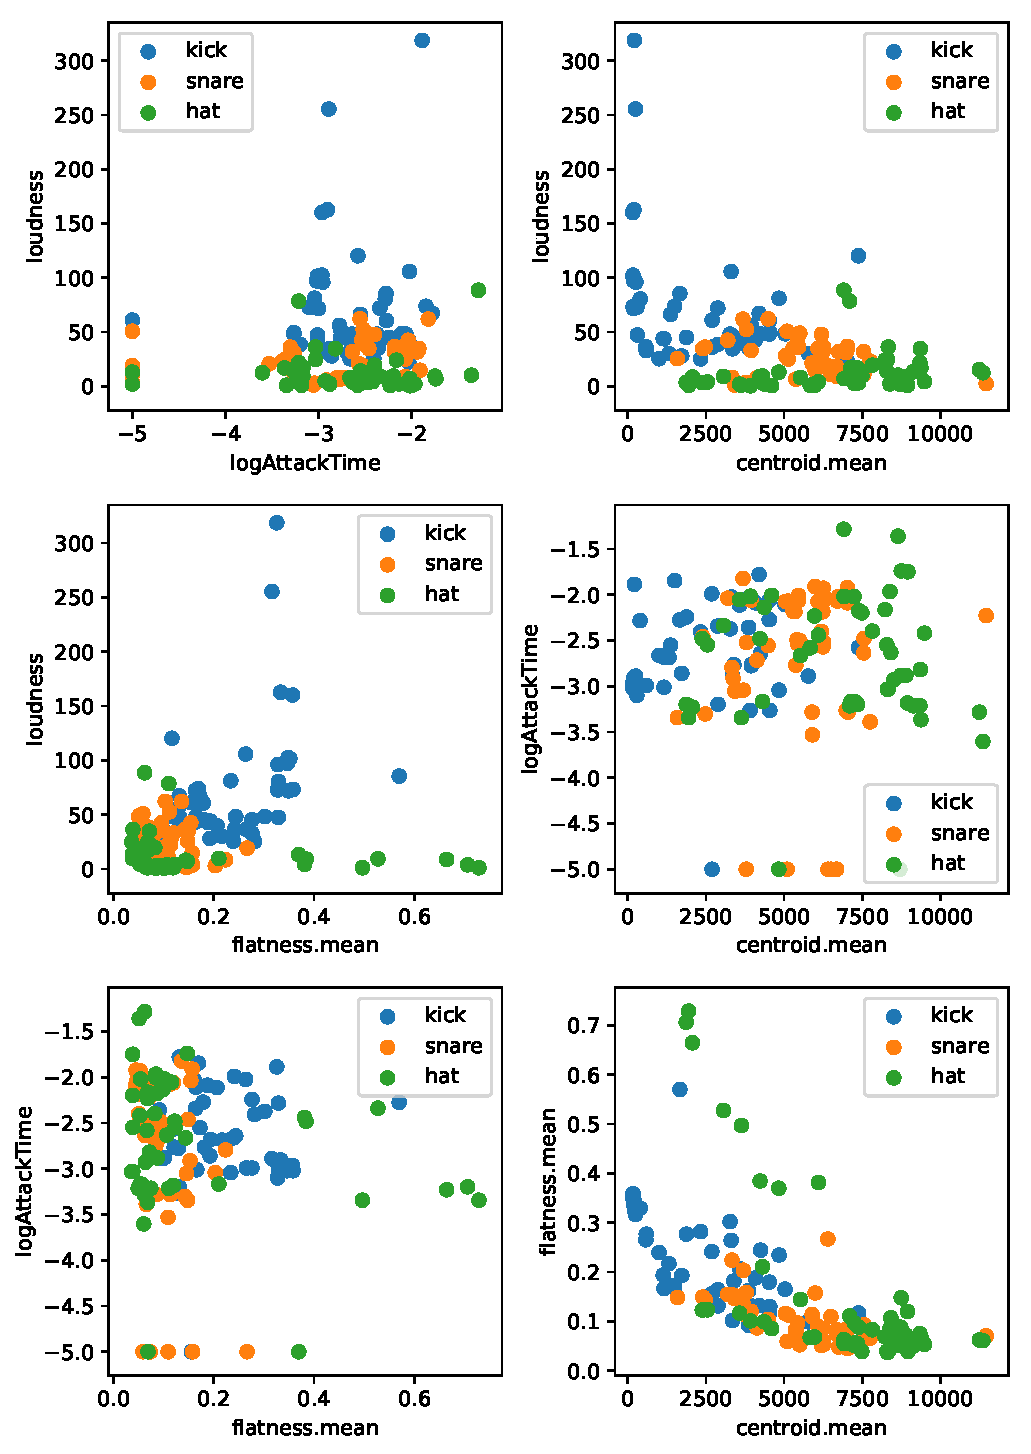
\includegraphics[width=1.0\textwidth]{ch06_rhythmcat/figures/feature_axis_combos.pdf}
	\end{center}
	\caption[Visualisation of all temporal and spectral feature combinations for kick, snare and hat drum sounds]{Visualisation of all temporal and spectral (taking the mean only) feature combinations for kick, snare and hat drum sounds}
	\label{fig:temporal_and_spectral_features}
\end{figure}


To address some of the shortcomings of visualisation based on raw singular feature values, it is often useful to apply some form of dimensionality reduction technique that can provide an `automatic' projection of the higher-order feature space into the timbre space suitable for visualisation of the data, while hopefully retaining most of the important trends latent within the data. Projections of higher order timbre spaces using dimensional scaling have been talked about in the literature for quite some time,  one of the key innovators in the usage of timbre spaces for creative or generative purposes has been David Wessel. By taking measurements of subjective responses to timbral stimuli, dimensionality reduction schemes are used to present a map of timbral references in space that can be then used to provide a spatial reference for generation and control of additive synthesis \citep{Wessel1979, Wessel1976}

Many dimensional reduction techniques span the literature as it is an important tool in general statistical analysis and machine learning. Specifically in the context of organising and exploring multimedia collections based on similarity, Christian Frisson's doctoral thesis \citeyearpar{frisson2015} offers a broad and up-to-date introduction to the main techniques and is a worthwhile reference. Here we summarise the principal methods that we have experimented with in our work.

\subsubsection{Principal Component Analysis}

\acrfull{pca} is a statistical procedure applied to data that can discover trends in order to preserve those with the most variance, effectively allowing us to compress data from high-dimensional space into lower-dimensional space without considerable ``loss'' of salience \citep{Hackeling2014}. Practical applications of \acrshort{pca} includes reducing redundant (features with low variance) data for more efficient machine learning tasks, and for producing coordinates that can make comparative visualisation of data possible in 2 or 3 dimensions.

It is the second application that interests us here, and in fact \acrshort{pca} has seen considerable application already in visualisation for musical applications \citep{Cooper2006}. Most of these involve organising large musical collections. Within the GiantSteps project, our colleagues have compared \acrshort{pca} with \acrshort{mds} (see below) 

\acrshort{pca} involves a few stages of matrix algebra and is implemented already in many libraries and frameworks so we won't concern ourselves with its derivation here. However the key stages are summarised in an excellent tutorial by \cite{Smith2002a}. Basically, the method uses eigenvalues and eigenvectors to extract the axes of maximum variance from the covariance matrix of the original data, and the highest eigenvectors are the principal components. As many principal components can be retained as required, with the assumption being that the loss will be minimal even as successively more components are discarded.

\subsubsection{Multidimensional Scaling}

\acrfull{mds} actually refers to a taxonomy of methods for dimensional reductions including `classical' or \acrfull{pcoa}, metric and non-metric \acrshort{mds}. \acrshort{mds} uses a distance or dissimilarity matrix as input and attempts to reduce the dimensions while preserving pairwise distance between entities, compared to \acrshort{pca} which tries to preserve maximum variance. \cite{frisson2015} puts it more succintly: ``\acrshort{mds} uses a distance matrix whereas \acrshort{pca} uses a correlation matrix.''.

Regarding musical applications, apart from the early experiments of Wessel, \citep{Wessel1976, Wessel1979} \acrshort{mds} has been used somewhat less than \acrshort{pca}. Within the GiantSteps project though, our colleagues have been studying the effects of symbolic rhythmic features on the organisation of symbolic rhythmic patterns in dance music when dimensionality reduction techniques such as \acrshort{pca}, \acrshort{mds} and \acrshort{tsne} (to follow) are applied \citep{Gomez-Marin2017, Gomez-Marin2016}. This expanded on previous perceptual dimensional scaling studies conducted by \cite{Gabrielsson1973a, Gabrielsson1973b} in the 1970s, who performed similarity ratings on  many parameters of rhythmic similarity of drum machine patterns and tried to find the most salient parameters that influenced the positioning of the patterns in a reduced \acrshort{mds} space.

\subsubsection{t-Distributed Stochastic Neighbour Embedding}

\acrfull{tsne} is a relatively recent prize-winning\footnote{\url{https://lvdmaaten.github.io/tsne/}} approach to data visualisation that is tailored specifically for effective reduction of high-dimensional datasets \citep{VanDerMaaten2008}. Based on a previous method known as \acrfull{sne}, one of the improvements it offers is  reductional strategies for preventing crowding or over-layered clusters in the centre of the map inherent in \acrshort{sne} methods. Essentially this is achieved by using a Student-t distribution rather than Gaussian for computing dissimilarity between points in low-dimensional space \citep{VanDerMaaten2008}.

The \acrshort{tsne} algorithm is gaining considerable favour in music information tasks as a way of navigating large collections of complex data representations \citep{Hamel2010, Grill2012, Frisson2014, Frisson2014a, Flexer2015, Martin2017, Font2017}. In a comparative evaluation of \acrshort{mds}, \acrshort{pca} and \acrshort{tsne} based on three criteria \cite{Dupont2013} revealed that t-SNE outranks PCA which in turn outranks \acrshort{mds} in three tasks related to musical loops and sound effects.

Returning to our own tasks of visualising feature vectors of drum sounds, \figref{fig:dimension_reductions} shows these three dimension reduction techniques applied to 50 instances each of kick, snare and hi-hat sounds based on the full gamut of features extrapolated with the GFCC+Spectral+Temporal configuration. One thing that's immediately apparent across all methods is their increased use of the 2-dimensional space in comparison to the individual assignment of features to axes as we saw in \figref{fig:temporal_and_spectral_features}, as well as exhibiting less crowding in overlapping clusters.

Most methods are quite capable of sorting the distinctive low frequency membrane kick sounds from the snares and hi-hats. There is, however, less separation of the more broadband cymbal and snare sound classes in both the \acrshort{mds} and \acrshort{pca} reduction methods. We see more overlapped clustering in the \acrshort{pca} method in this instance, but in other reduction experiments this has often been reversed. In an ideal world a concatenative system would have some trained mechanism for performing all three procedures then choosing the one with the best separation.

\begin{figure}
	\begin{center}
		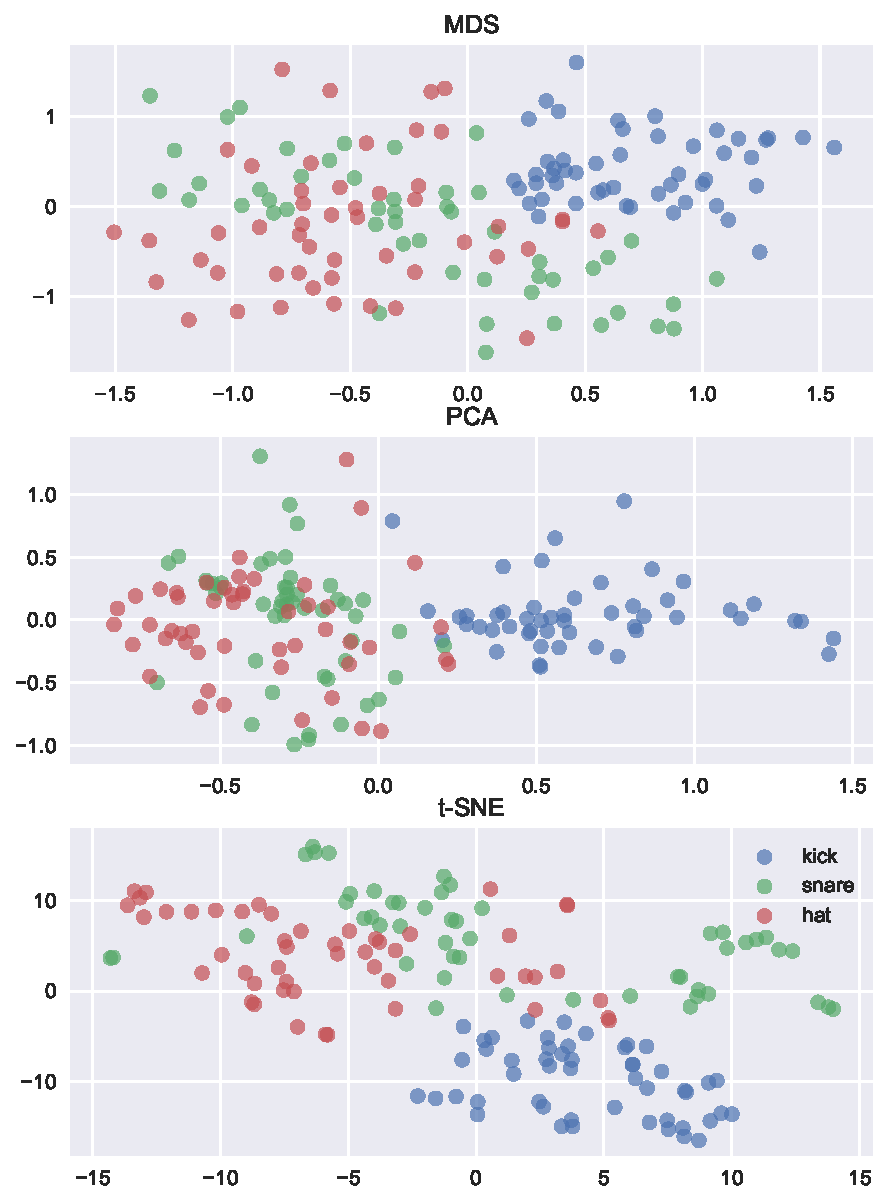
\includegraphics[width=1.0\textwidth]{ch06_rhythmcat/figures/dimension_reductions.pdf}
	\end{center}
	\caption[MDS, PCA and t-SNE Dimension Reduction on Kick,Snare and Hat Sounds]{\acrshort{mds}, \acrshort{pca} and \acrshort{tsne} dimension reduction processes applied to kick, snare and hi-hat sounds}
	\label{fig:dimension_reductions}
\end{figure}

\subsubsection{Interacting with Sounds and Creating a Metaphor}

Undoubtably, the timbre space paradigm represent a much richer modality for organising sound spatially and a provides a vital window into understanding the procedures governing concatenative synthesis. We have seen how exactly rendering these spaces is not trivial and it poses a unique set of challenges and tradeoffs to get a usable and meaningful landscape for exploration.

Equally challenging, once a timbre space has organised a visual map of sound, is how to \textit{interact} with those sounds. How can the user effectively navigate this sonic terrain and avail of suitable gesture and metaphor to arrange the sounds in the desired manner? How do existing concatenative synthesis deal with these challenges? To complicate matters further, our system is inherently rhythm driven. How do those sound exploratory devices extend to our unique problem domain?

In CataRT the primary interaction metaphor is simple and intuitive: the target is the real-time position of the mouse cursor and a resizable radar around the target filters the range of sounds within its proximity. How these sounds are triggered depends on the mode selected. The triggering modes include:

\begin{itemize}
  \item \textit{Bow} - trigger closest unit each time you move the mouse
  \item \textit{Fence} - like a stick dragging along a fence, triggers when a new unit becomes closer to the target
  \item \textit{Beat} - triggers according to metronome
  \item \textit{Chain} - triggers after previous unit finishes
  \item \textit{Quant} - non-functional quantised mode
  \item \textit{Seq} - trigger via external sequencer
  \item \textit{Cont} - play back units in order
\end{itemize}

In earGram the SpaceMap mode also triggers units based on proximity to the mouse pointer target, but defines three different triggering modes distinct from CataRT:

 \begin{itemize}
  \item \textit{continuousPointer} - continuously play units at a specified rate
  \item \textit{pointerClick} - same as continuousPointer but ``played in response to a controller command'' (the meaning of this is not exactly clear from the description provided)
  \item \textit{colorPicker} - selects units based on colours. 
  \item \textit{liveInput} - feature analysis of live input sets pointer position.
\end{itemize} 

AudioGarden appears to adapt the mouse radar approach of CataRT also, but the positioning of multiple radars in the timbre space means multiple grains can be triggered for a single target unit in time which is a very simple and useful method of mixing corpus units vertically in addition to concatenating them horizontally.

\subsection{A Prototypical Rhythmic Concatenative Synthesiser Interface}

\subsubsection{First Iteration}

Our first attempt at a prototype interface that was capable of performing rudimentary rhythm-driven concatenative synthesis was naturally extremely crude and experimental (\figref{fig:rhythmcat_proto1}) but a valuable learning experience and necessary stepping stone.

\begin{figure}
	\begin{center}
		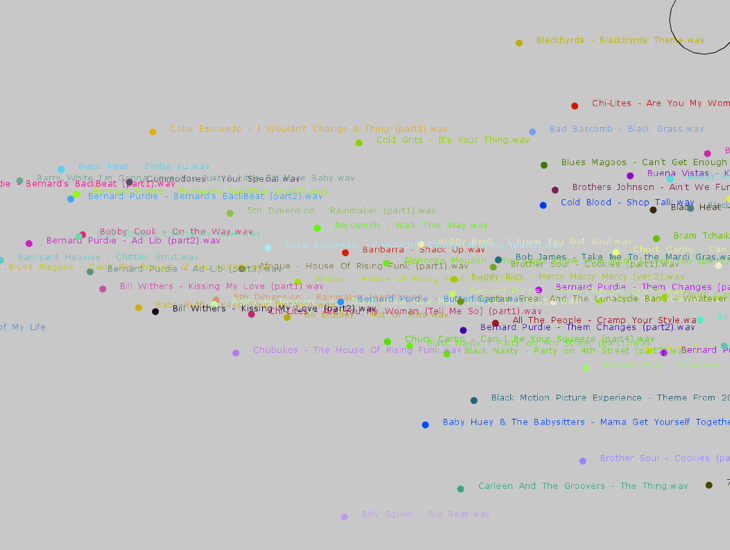
\includegraphics[width=1.0\textwidth]{ch06_rhythmcat/figures/rhythmcat_proto1.png}
	\end{center}
	\caption[RhythmCAT First Prototype]{RhythmCAT First Prototype. Entire waveforms are represented in space using \acrshort{pca} reduction of the \acrshort{mfcc}. A small mouse radar scans the space and onsets are played at random from the files in proximity.}
	\label{fig:rhythmcat_proto1}
\end{figure}

Developed in openFrameworks\footnote{\url{http://openframeworks.cc/}}, the application used \acrshort{mfcc} features computed on the entire audio file, then positioned the sound in space (along with its filename string for some reason which now evades me!) according to \acrshort{pca} reduction of the features. To explore the sounds we adapted the radar style navigation metaphor introduced in CataRT, but this immediately raised the question of how to trigger the sounds. This early incarnation simply selected an onset chosen at random from within radar proximity to the mouse target and triggered at each beat according to a 1/16 grid subdivision of the tempo.

\subsubsection{Second Iteration}

The next iteration was largely concerned with implementation. We reasoned that the typical dance music producer would not use software like this unless it was integrated into their existing workflow of tools, meaning we needed to consider how interface it with a \acrshort{daw} like Ableton. So, we spent some time developing a streaming real-time plugin using \acrfull{vst} that could synchronise with the tempo information received from a \acrshort{vst}-host enabled \acrshort{daw}, and also allow the user to select different beat subdivisions.

\begin{figure}
	\begin{center}
		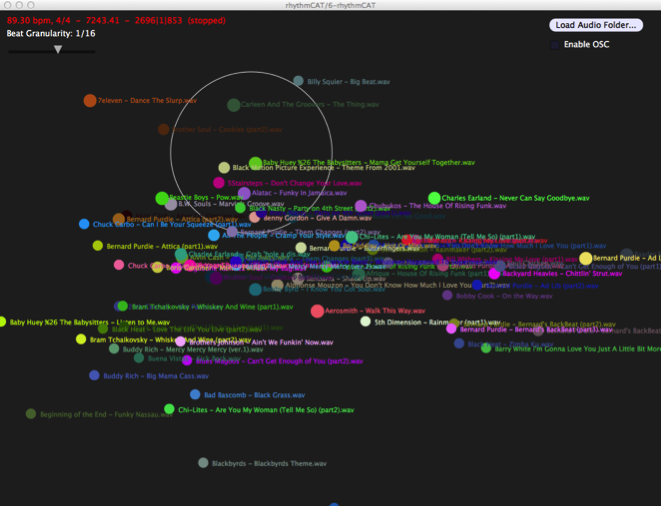
\includegraphics[width=1.0\textwidth]{ch06_rhythmcat/figures/rhythmcat_proto2.png}
	\end{center}
	\caption[RhythmCAT First Prototype]{RhythmCAT Second Prototype, implemented as a \acrshort{vst} plugin}
	\label{fig:rhythmcat_proto1}
\end{figure}

While this version was more streamlined and featured a slicker interface built with the aid of JUCE, fundamentally it performed the same functionality. The points in space referred to complete sound files and a mouse radar filtered the points by proximity. Targeting could be controlled by external systems via the \acrshort{osc} or automatically and algorithmically using Boids \citep{Reynolds1987}, a flocking algorithm that has been used in other systems for controlling spatialisation and granulation parameters in electroacoustic works.\citep{Kim-Boyle2006, Wilson2008, Barreiro2010}. 

But these are arbitrary and deferential extensions that still just scrub the surface features of  the visual space. Using the tool as a rhythm generation tool reveals the deficiency of the mouse radar exploratory method. A typical drum pattern is made up of complementary sounds in different timbres and hence occupy different zones of the timbre space at different points in time. This is conceivably better served by the multi circle model of \citep{Frisson2010}'s AudioGarden, which could be used to place three circles in the timbre space corresponding to the kick, hat and snare, as an example.

Most critically, these prototypes did not yet integrate the possibility of an audio target could  intelligently define where the system should search for units to select. We will will now discover how these two outstanding concerns are resolved by adapting a graph model, inspired by the modular metaphor, that shows the spatial connection and temporal evolution between consecutive units selected for concatenation, in the breadth and span of a timbre space, given a target sound specification.

\section{RhythmCAT}

Building on all the topics we have been discussing in this dissertation, RhythmCAT was conceived as ``a user-friendly system for generating rhythmic loops that model the timbre and rhythm of an initial target loop'' \citep{Nuanain2017b}. This system was first introduced at \acrfull{nime} in 2016 \citep{Nuanain2016a}, subsequent papers dealt with its evaluation \citep{Nuanain2016b, Nuanain2016c} culminating in a summary journal article for the Computer Music Journal in 2017 \citep{Nuanain2017b}.

%\subsection{Identifying our Users}
%
%<TODO - TALK ABOUT MUSIC PRODUCERS, RED BULL ETC>
%
%\subsection{Real-time Challenges}
%
%<TODO - EXPLAIN CHALLENGES WITH HMM AND REAL-TIME>

\subsection{Developing the System}

In this section, we will describe our implementation of the RhythmCAT system, beginning with an explanation of the musical analysis stages of onset detection, segmentation and feature extraction. This is followed by an examination of the interactive user interface and the pattern generation process. \figref{fig:rhythmcat_flowchart} gives a diagrammatic overview of these important stages, which can be briefly summarised as:

\begin{enumerate}
  \item Sound Input
  \item Onset Detection \& Segmentation
  \item Audio Feature Extraction
  \item Storage \& Data Representation
  \item Pattern Synthesis
  \item Real-time Audio Output
\end{enumerate}

\begin{figure}
	\begin{center}
		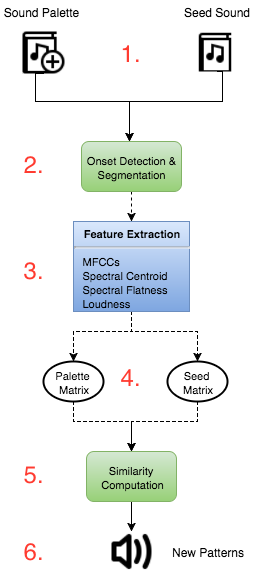
\includegraphics[width=0.6\textwidth]{ch05_pyconcat/figures/rhythmcat_flowchart.png}
	\end{center}
	\caption[Block Diagram of Functionality in RhythmCAT System]{Block Diagram of Functionality in RhythmCAT System}
	\label{fig:rhythmcat_flowchart}
\end{figure}

The system is developed in C++ using the JUCE framework \footnote{\url{https://juce.com/}}, the Essentia musical analysis library \citep{Bogdanov2013} and the OpenCV computer vision library \citep{Bradski2000} (for matrix operations an \acrshort{pca}).
 
\subsubsection{Sound Input}

The first stage in building a concatenative music system generally involves gathering a database of sounds to select from during the synthesis procedure. This database can be manually assembled but in many musical cases the starting point is some user-provided audio that may range in length from individual notes to phrases to complete audio tracks.
 
The two inputs to the system are the Sound Palette and the Seed Sound. The sound palette refers to the pool of sound files we want to use as the sample library for generating our new sounds. The seed sound refers to the short loop that we wish to use as the similarity target for generating those sounds. The final output sound is a short (one to two bars) loop of concatenated audio that is rendered in real time to the audio host.

\subsubsection{Onset Detection and Segmentation}

In cases where the sounds destined for the sound palette exceed note or unit length, the audio needs to be split into its constituent units using onset detection and segmentation.

We covered onset detection methods at length in \chapref{chap:pyconcat}, and we showed how how the most accurate methods come at a cost of increased computational complexity, especially when involving the use of state of the art deep learning techniques. What's more, the \acrshort{cnn} algorithm is only available in the Python Madmom library, which excludes it from being a possible method in our compiled and monolithic plugin at the present time. A port of Superflux is available in Essentia, but for best results it requires considerable tweaking of the parameters that depends heavily on the program material to be analysed, meaning it was quite hard to find a generalised configuration to cover a wide range of possible input sounds to the instrument. 

To this end we rely on the standard `OnsetRate' method that at least returned acceptable results when concentrated on the percussive datasets used in the evaluation (\tabref{tab:extended_onset_statistics}). As a reminder this invoked two methods based on analysing signal spectra from frame to frame (at a rate of around 11 ms). The first method involves estimating the high-frequency content in each frame \citep{Masri1996} while the second method involves estimating the differences of phase and magnitude between each frame \citep{Bello2005}.

The onset detection process produces a list of onset times for each audio file, which we use to segment into new audio files corresponding to unit sounds for our concatenative database.

\subsubsection{Audio Feature Extraction}

As stressed, successful feature extraction is a tradeoff between choosing the richest set of features capable of describing the signal succinctly at the expense of storage and computational complexity. This is more important than ever in the design of a real-time instrument such as here. Whereas the PyConcat environment offered powerful selection and combination of a wide set of descriptors, RhythmCAT has a smaller subset that is more manageable complexity wise. These features are as follows, along with their intended perceptual label.
 
 \begin{itemize}
  \item \textbf{Power} - computed using Stevens' Law to estimate "Loudness".
  \item \textbf{Spectral Centroid} - for estimating "Brightness".
  \item \textbf{Spectral Flatness} - for estimating "Harmonicity".
  \item \textbf{*FCC [2-13]} - for abstracting "Timbre". At the moment we use regular \acrshort{mfcc} as our implementation of \acrshort{bfcc} has not been fully optimised and is slightly slower.
\end{itemize}

\subsubsection{Pattern Synthesis and User Interaction}

Further on we will describe a bit more on how the seed or target audio signal is actually received from the \acrshort{vst} host, but in terms of analysis on that seed signal, the process is the same as before: onset detection and segmentation followed by feature extraction.

The resulting feature vectors are stored in two matrices: the palette matrix and the target matrix. The palette matrix stores the feature vectors of each unit of sound extracted from the sound palette and similarly the target matrix stores feature vectors of units of sound extracted from the seed loop.

\subsubsection{Pattern Synthesis}

This section details the visible, aural and interactive elements of the system as they pertain to the user. \figref{fig:rhythmcat_interface} gives a glimpse of the user interface in a typical pattern generation scenario.

\begin{sidewaysfigure}
	\begin{center}
		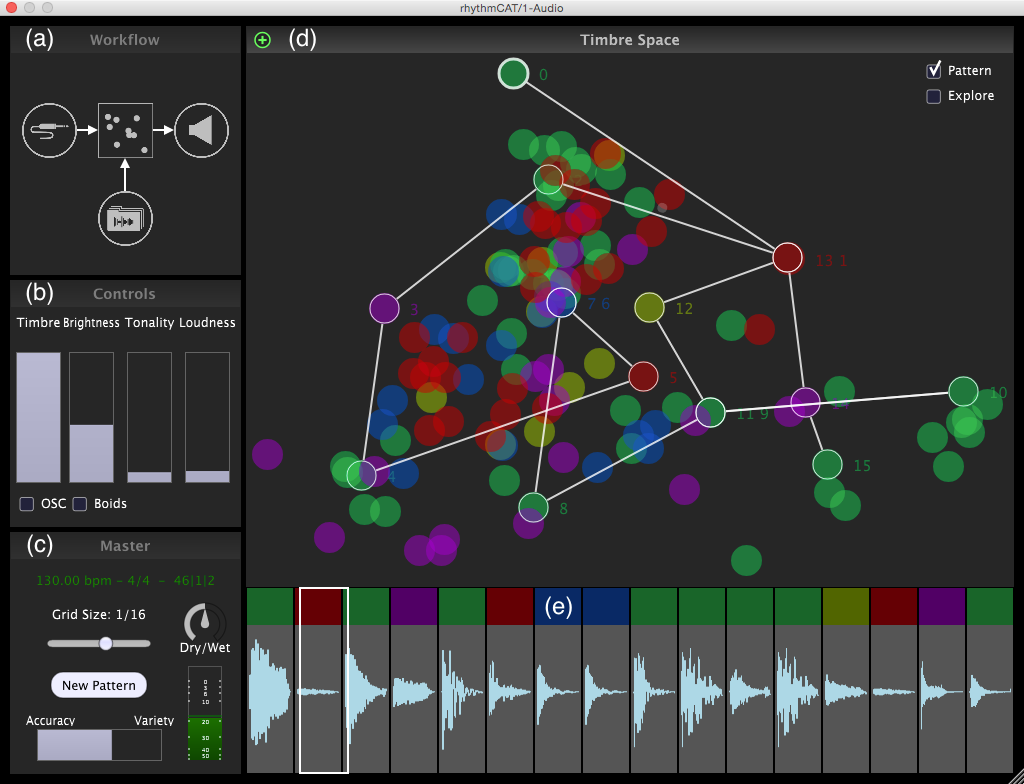
\includegraphics[scale=0.45]{ch05_pyconcat/figures/rhythmcat.png}		
		\end{center}
		\caption[Main User Interface Showing Panels A-E with Onset Graph]{Main User Interface Showing Panels A-E with Onset Graph}
	\label{fig:rhythmcat_interface}
\end{sidewaysfigure}

\paragraph{Workflow}

The layout of the interface was the result of a number of iterations of testing with users who, while praising the novelty and sonic value of the instrument, sometimes expressed difficulty understanding the operation of the system. One of the main challenges faced was how best to present to the user the general workflow in a simple and concise manner. It was decided to represent the flow of the various operations of the software emphatically by using a simple set of icons and arrows, as is visible in \figref{fig:rhythmcat_interface}.

%\begin{figure}
%	\begin{center}
%		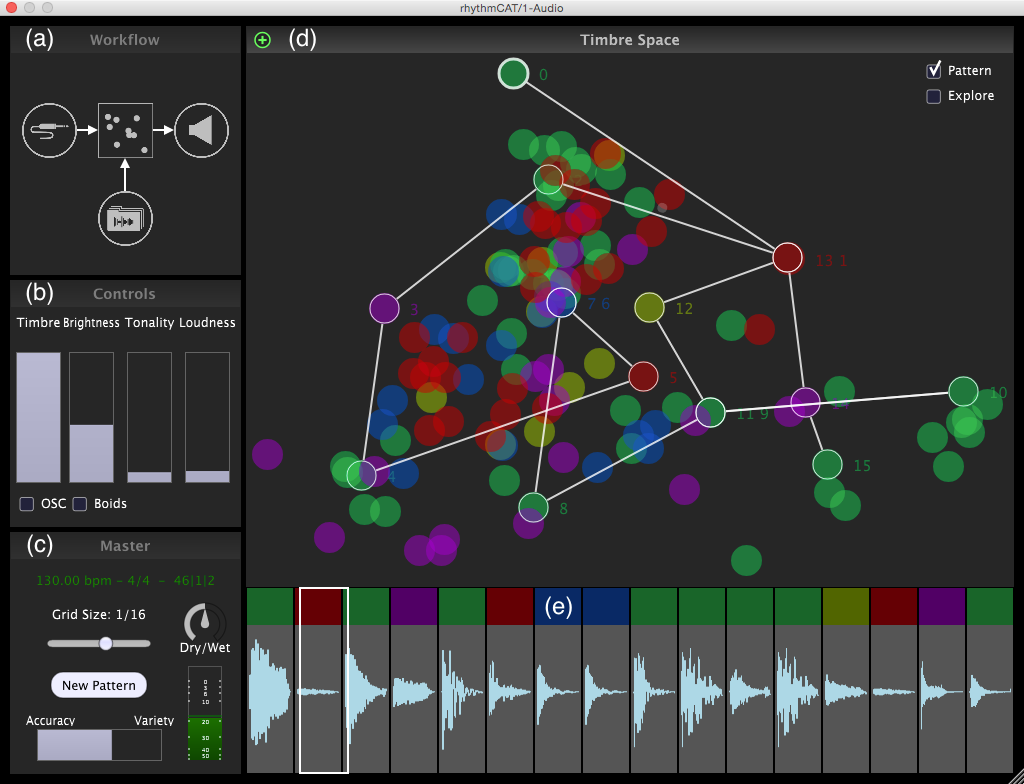
\includegraphics[width=1.0\textwidth]{ch05_pyconcat/figures/rhythmcat.png}
%	\end{center}
%	\caption[Main User Interface Showing Panels A-E with Onset Graph]{Main User Interface Showing Panels A-E with Onset Graph}
%	\label{fig:rhythmcat_interface}
%\end{figure}
 
The icons indicate the four main logical operations that the user is likely to do, and opens up the related dialogs, namely:
\begin{itemize}
  \item The Palette Dialog - as indicated by the folder icon
  \item The Seed Dialog - as indicated by the jack cable icon
  \item The Sonic Dialog - as indicated by the square feature space icon
  \item The Output Dialog - as indicated by the speaker icon
\end{itemize}

\paragraph{Sound Palette}

The user loads a selection of audio files, or folders containing audio files, which are analysed to create the sound palette as has previously been discussed. Next, dimensionality reduction is performed on each feature vector of the units in the sound palette using \acrfull{pca}. Two \acrshort{pca} components are retained and scaled to the visible area of the interface to serve as coordinates for placing a circular representation of the sound in two-dimensional space. These visual representations, along with their associated audio content, we term sound objects. They are clearly visible in main timbre space window in the figure.

\paragraph{Seed Input}

Seed audio is captured and analysed by recording directly from the input audio of the track on which the instrument resides in the audio host. Using the real-time tempo and bar/beat information provided by the host, the recorder will wait until the next bar starts to begin capture, and will only capture complete bars of audio. This audio is analysed as before but with one exception. Since the goal of the instrument is to integrate with an existing session and generate looped material, we make the assumption that the incoming audio is quantised and matches the tempo of the session. Thus, onset detection is not performed on the seed input; rather, segmentation takes place at the points in time determined by the grid size (lower left of the screen).

An important aspect to note: since the instrument is fundamentally real-time in its operation, we need to be careful about performing potentially time consuming operations such as feature extraction when the audio system is running. Thus, we perform the audio recording stage and feature extraction process on separate threads so the main audio playback thread is uninterrupted. This is separate to yet another thread that handles elements of the user interface.

\paragraph{Sonic Parameters}

Clicking on the square sonic icon in the centre of the workflow component opens up the set of sliders shown in (\figref{fig:rhythmcat_interface} -B) that allows us to adjust the weights of the features in the system. Adjusting these weightings has effects in terms of the pattern generation process but also in the visualisation. Presenting their technical names (centroid, flatness and \acrshort{mfcc}s) would be confusing for the general user, thus we have relabelled them with what we consider their most descriptive subjective labelling. With the pattern generation process, these weights directly affect the features when performing similarity computation and unit selection, as we will see in the next section. Depending on the source and target material, different combinations of feature weightings produce noticeably different results. Informally we have experienced good results using \acrshort{mfcc}s alone for example, as well as combinations of the flatness and centroid. In terms of visualisation, when the weights are changed, dimensionality reduction is re-initiated and hence positioning of the sound objects in the timbre space changes. Manipulating these parameters can help disperse and rearrange the sound objects for clearer interaction and exploration by the user in addition to affecting the pattern generation process.

Once the palette and seed matrices have been populated, a similarity matrix between the palette and seed matrix is created. Using the feature weightings from the parameter sliders, a sorted matrix of weighted Euclidean distances between each onset in the target matrix and each unit sound in the palette matrix is computed as per \eqnref{eq:linear_search} in \chapref{chap:pyconcat}

\paragraph{Unit Selection}

In \chapref{chap:pyconcat} we summarised the various unit selections ranging from the basic linear search procedure to Viterbi style decoding. We then proposed two novel unit selection methods that expand Viterbi decoding further to produce a \textit{k}-Best list of potential sequences for exploring variations.

While these methods provide increasingly richer and more interconnected syntheses of a target sound, the complexity increases and the performance suffers, as we saw in the analysis of the two \textit{k}-Best methods. Evidently this poses problems for real-time scenarios, as  Coleman has noticed:

\blockcquote[]{Coleman2015}{``\textit{None of the systems cited in this section use advance planning by minimizing transition costs (in contrast to some of the systems [...], i.e. Caterpillar, Musaicing, or Audio Analogies). This is likely due to its high computational cost. Instead, more immediate selection methods are used.}''}

Which reiterates an earlier remark by Schwarz with regards to CataRT:

\blockcquote[]{Schwarz2006b}{``\textit{Because of the real-time orientation of CataRT, we cannot use the globally optimal path-search style unit selection based on a Viterbi algorithm as in Caterpillar, neither do we consider concatenation quality, for the moment. Instead, the selection is based on finding the units closest to the current position x in the descriptor space, in a geometric sense...}''}

So this likely rules out the Viterbi decoding methods we have described, even though we should emphasise that our tool is not strictly real-time - in the sense that it computes complete loops based on the analysis of one bar in a given tempo in order to capture a temporal context - thus we would qualify it as \textit{quasi} real-time. Regardless, for performance, in RhythmCAT we only consider the target cost when concatenating output sequences, thus making its unit selection scheme a variation on linear search. While we do sacrifice the continuity factor that is inherent in Viterbi decoding, when considered, it might not hold the same sway for rhythm purposes as it would for synthesising voice or solo instrument performance. Given that a kick and snare have, or should have, very different spectral and timbre profiles, efforts to constrain the slope of features between them should really only concentrate on ensuring some consistency of energy\footnote{In the absence of any magical timbre feature analysis techniques that we know of that can be used to isolate and ensure unit selection comes from similar timbre of just the room profile, recording chain or album and not the instrument timbre, or in other words, only retaining those features that contribute to the `album effect'\citep{mandel2005song, kim2006towards}}.

The unit selection algorithm is quite straightforward, and to allow for flexible exploration of variations instead of returning the nearest neighbour sequence we allow any mixing and matching of units from the corpus sorted by similarity to the targets. For each unit $i$ in the segmented target sequence (e.g. 16-step) and each corpus unit $j$ (typically many more), the target unit cost $C_i,j$ is calculated by the weighted Euclidean distance of each feature $k$ as per usual.

These unit costs are stored in similarity matrix $M$. Next we create a matrix $M’$ of the indices of the ascendingly sorted elements of $M$. Finally, a concatenated sequence can be generated by returning a vector of indices $I$ from this sorted matrix and playing back the associated sound file. To retrieve the closest sequence $V_0$ one would only need to return the first row.

Returning sequence vectors as rows of a (sorted) matrix limits the number of possible sequences to the matrix size. This can be extended if we define a similarity threshold $T$ and return a random index between $0$ and $j − T$ for each step $i$ in the new sequence.

\paragraph{Pattern Generation and Interaction}

In our description of the early prototypes we highlighted the challenge of coming up with an effective visualisation and interaction paradigm that could show the map of sounds in timbre space as well as the temporal evolution and connection of a rhythmic-centric concatenated sequence that makes its way through that timbre space in accordance to some target. The interaction metaphor we propose to tackle this is to represent a rhythm as a path through that graph or network, with edges connecting each sound in space as appropriate. This obviously borrows heavily from the Modular metaphor explained at the chart of the chapter and \citep{Roma2010} uses a similar graph grammar style metaphor for navigating the Freesound\footnote{\url{https://freesound.org/}} library. More recently, \cite{Font2017} proposes a similar tool for the same task that uses the \acrshort{tsne} reduction method to arrange samples.

Facilitating the efficient \acrshort{ui} visualisation and interaction of sequences of units in space is enabled with the use of a linked list data structure to contain the necessary information of each unit. Linked lists, as explained in any introductory text on data structures are an efficient way of ordering data in a linear fashion and is an apt container for chaining the series of nodes in our graph model.

To create a pattern when the user hits the ``New Pattern'' button (\figref{fig:rhythmcat_interface} - C), a new linked list of objects we term sound connections is formed, representing a traversal through connected sound objects in the timbre space. The length of the linked list is determined by the grid size specified by the user, thus if the user specifies a grid size of 1/16 for example, a one bar sequence of 16th notes will be generated. The exact procedure whereby we generate a list is detailed in Algorithm \ref{alg:sequential_scan_lower_bound}. The variance parameter affects the threshold of similarity by which onsets are chosen. With 0 variance, the most similar sequence is always returned. This variance parameter is adjustable from the Accuracy/Variety slider in the lower left corner of the instrument (\figref{fig:rhythmcat_interface} - C).

\begin{algorithm}
	\caption{Get Onset List for Concatenative Sequence}
	\label{alg:sequential_scan_lower_bound}
	\begin{algorithmic}
		\For {n in GridSize}
			\State R = Random number 0 < Variance
			\State I = Index from Row R of Similarity Matrix
			\State S = New SoundConnection
			\State S->SoundUnit = SoundUnit(I)
			\State Add S to Linked List
		\EndFor
		\\
	\Return	LinkedList	
	\end{algorithmic}
\end{algorithm}
 
In the main timbre space interface (\figref{fig:rhythmcat_interface} - D), a visual graph is generated in the timbre space by traversing the linked list and drawing line edges connecting each sound object pointed to by the sound connection in the linked list. In this case a loop of 16 onsets has been generated, with the onset numbers indicated beside the associated sound object for each onset in the sequence. An animated trace shows the units triggered in time with each beat of the tempo source from the \acrshort{vst} host. Of course the most compelling aspect of this is that the user is free to manipulate these sound connections to mutate these patterns by touching or clicking on the sound connection and dragging to another sound object. Multiple sound connections assigned to an individual sound object can be group selected by double tapping then dragging, useful for changing all instances of a hi-hat or a snare for example

On the audio side, every time there is a new beat, the linked list is traversed and if a sound connection's onset number matches the current beat the corresponding sound unit is played back. One addition that occurred after some user experiments (see \chapref{chap:evaluation}) with the prototype is the linear waveform representation of the newly generated sequence \figref{fig:rhythmcat_interface} - E). Users felt the combination of the 2D interface with the traditional waveform representation made the sequences easier to parse visually as well as being able to manipulate the internal arrangement of sequence itself once generated.

%\subsubsection{Improvements for User-Driven Concatenative Synthesis}
%
%Real-time Pitch Quantisation Techniques and Time Alignment